\documentclass[12pt,french]{article}
\usepackage[utf-8]{inputenc}
\usepackage[T1]{fontenc}
\usepackage{babel}
\usepackage[margin=2cm]{geometry}
\usepackage{graphicx}
\usepackage{xcolor}
\usepackage{listings}
\usepackage{hyperref}
\usepackage{fancyhdr}
\usepackage{tikz}
\usepackage{booktabs}

% Couleurs
\definecolor{darkblue}{rgb}{0.1,0.2,0.5}
\definecolor{lightgray}{rgb}{0.95,0.95,0.95}

% En-tête
\pagestyle{fancy}
\fancyhf{}
\fancyhead[C]{\textbf{Tradrly Bot - Résumé des Travaux}}
\fancyfoot[C]{\thepage}

% Configuration listings
\lstset{
    language=bash,
    basicstyle=\ttfamily\small,
    backgroundcolor=\color{lightgray},
    breaklines=true,
    keywordstyle=\color{darkblue}\bfseries,
    commentstyle=\color{gray},
    stringstyle=\color{red},
    breakatwhitespace=false,
    frame=single,
    rulecolor=\color{darkblue}
}

\title{\textbf{\Large TRADRLY BOT}\\{\small Assistant Productivité - Application Desktop}}
\author{Bouthaina Rjaibi}
\date{Juin 2026}

\begin{document}

\maketitle

\section*{1. Vue d'ensemble du projet}

\textbf{Tradrly Bot} est une application desktop intelligente conçue pour :
\begin{itemize}
    \item Analyser des commandes en français naturel
    \item Extraire intentions, entités et priorités
    \item Gérer tâches, événements et sessions de focus
    \item Fournir une interface utilisateur intuitive avec CommandBar
\end{itemize}

\vspace{0.5cm}

\section*{2. Stack Technologique}

\begin{table}[h!]
\centering
\begin{tabular}{lll}
\toprule
\textbf{Couche} & \textbf{Technologie} & \textbf{Port/Rôle} \\
\midrule
Frontend & React 18 + TypeScript & Vite (5173) \\
Desktop & Electron 42.4.1 & Application native \\
Backend (Node) & Express 4.18 & API REST (3001) \\
Backend (Python) & FastAPI + SQLAlchemy & NLP (8000) \\
NLP & Spacy 3.5 + TextBlob + NLTK & Traitement texte \\
Base de données & SQLite & Stockage local \\
\bottomrule
\end{tabular}
\end{table}

\vspace{0.5cm}

\section*{3. Fonctionnalités Implémentées}

\subsection*{3.1 Interface Intelligente (React)}
\begin{itemize}
    \item \textbf{CommandBar} : Saisie texte avec analyse NLP en temps réel
    \item \textbf{ProductivityHome} : Hub central avec modules modulaires
    \item \textbf{TasksView amélioré} : Entrée intelligente avec analyse NLP complète
    \item \textbf{Affichage intents} : Code couleur par catégorie (create\_task, create\_event, etc.)
    \item \textbf{Design responsive} : Adaptation desktop 1280×820px
\end{itemize}

\subsection*{3.2 Traitement NLP (Python)}
\begin{itemize}
    \item \textbf{NER (Named Entity Recognition)} : Extraction personnes, organisations, lieux, projets
    \item \textbf{POS Tagging} : Identification verbes d'action (créer, ajouter, démarrer, etc.)
    \item \textbf{Dépendances syntaxiques} : Extraction objet direct et contexte
    \item \textbf{Priorités} : Scoring 1-5 (urgent, important, normal, faible, très faible)
    \item \textbf{Sentiments} : Polarité et subjectivité via TextBlob
    \item \textbf{Participants} : Extraction assignés et collaborateurs
    \item \textbf{Deadlines} : Parsing de dates en français naturel
\end{itemize}

\subsection*{3.3 TasksView Intelligente (Nouveau)}
\begin{itemize}
    \item \textbf{Saisie naturelle} : Décris ta tâche en français libre (ex: "Appeler Alice demain 14h URGENT")
    \item \textbf{Analyse temps réel} : Affiche intention, priorité, participants, deadline au fur et à mesure
    \item \textbf{Métadonnées auto-extraites} :
    \begin{itemize}
        \item Priorité (1-5) avec couleur (rouge=urgent, orange=important, etc.)
        \item Participants extraits automatiquement
        \item Deadline parsée en format lisible (📅 18 juin 2026)
    \end{itemize}
    \item \textbf{Interface améliorée} :
    \begin{itemize}
        \item Checkbox pour cocher/décocher tâches (✅/⭕)
        \item Affichage priorité colorée pour chaque tâche
        \item Métadonnées visibles (assigné, deadline)
        \item Stats par priorité (Urgent, Important, Normal)
    \end{itemize}
    \item \textbf{Historique des actions} : Log des tâches créées avec métadonnées extraites
\end{itemize}

\subsection*{3.4 Endpoints API}
\begin{table}[h!]
\centering
\begin{tabular}{lll}
\toprule
\textbf{Endpoint} & \textbf{Méthode} & \textbf{Description} \\
\midrule
\texttt{/api/parse-intent} & POST & Route vers FastAPI (analyse NLP) \\
\texttt{/productivity/analyze} & POST & Analyse complète NLP (backend) \\
\texttt{/api/execute} & POST & Exécute commandes système \\
\bottomrule
\end{tabular}
\end{table}

\vspace{0.5cm}

\section*{4. Exemple de Flux - Commande Utilisateur}

\subsection*{TasksView Intelligente}
\begin{lstlisting}
# Utilisateur tape dans le champ de tâche
"Appeler Alice demain 14h URGENT"

# Analyse NLP en temps réel affiche:
Intent: create_task
Priorité: 🔴 URGENT (5)
Avec: Alice
Deadline: 18 juin 2026

# Utilisateur clique "Ajouter"
Tâche créée: "Appeler Alice demain 14h" [URGENT]
- Affichée avec priorité rouge
- Assigné: Alice
- Deadline: 📅 18 juin 2026

# Stats mises à jour
Total: 3 | Todo: 2 | Done: 1 | Urgent: 1
\end{lstlisting}

\subsection*{Exemples d'Entrées Naturelles}
\begin{itemize}
    \item \textit{"Finir le dashboard avant vendredi"} → Tâche avec deadline vendredi, priorité normal
    \item \textit{"Réunion avec Bob et Carol lundi 10h URGENT"} → Deadline lundi, participants Bob \& Carol, priorité urgent
    \item \textit{"Appels clients IMPORTANT"} → Tâche sans deadline, priorité important
    \item \textit{"Lunch avec Sarah demain 12h"} → Deadline demain, participant Sarah, priorité normal
\end{itemize}

\vspace{0.5cm}

\section*{5. Architecture Système}

\begin{center}
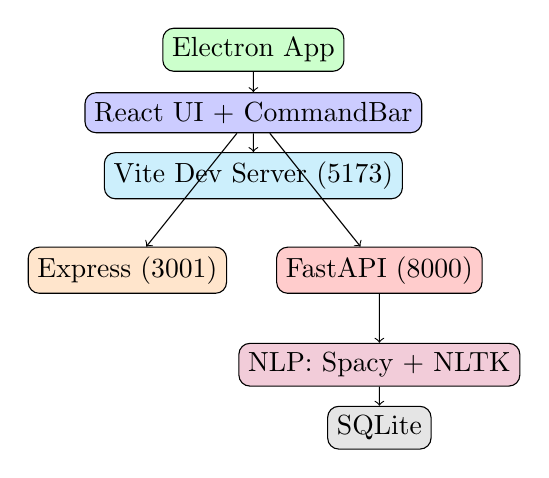
\begin{tikzpicture}[scale=0.8, every node/.style={draw, rectangle, rounded corners}]
  \node (electron) at (2, 4) [fill=green!20] {Electron App};
  \node (react) at (2, 3) [fill=blue!20] {React UI + CommandBar};
  \node (vite) at (2, 2) [fill=cyan!20] {Vite Dev Server (5173)};
  
  \node (express) at (0, 0.5) [fill=orange!20] {Express (3001)};
  \node (fastapi) at (4, 0.5) [fill=red!20] {FastAPI (8000)};
  \node (nlp) at (4, -1) [fill=purple!20] {NLP: Spacy + NLTK};
  \node (db) at (4, -2) [fill=gray!20] {SQLite};
  
  \draw[->] (electron) -- (react);
  \draw[->] (react) -- (vite);
  \draw[->] (react) -- (express);
  \draw[->] (react) -- (fastapi);
  \draw[->] (fastapi) -- (nlp);
  \draw[->] (nlp) -- (db);
\end{tikzpicture}
\end{center}

\vspace{0.5cm}

\section*{6. Commandes de Démarrage}

\subsection*{Mode Développement (Complet)}
\begin{lstlisting}
npm run electron:dev
# Lance concurrently:
# - Express server (3001)
# - Vite dev server (5173)
# - Electron app
\end{lstlisting}

\subsection*{Backend Python NLP}
\begin{lstlisting}
cd productivity_api
pip install -r requirements.txt
python setup_nlp.py      # Télécharge modèles Spacy/NLTK
uvicorn main:app --reload --port 8000
\end{lstlisting}

\vspace{0.5cm}

\section*{7. Sécurité \& Qualité}

\begin{itemize}
    \item \textbf{Vulnérabilités npm} : 0 (audit npm clean)
    \item \textbf{Erreurs TypeScript} : 0 (build réussi)
    \item \textbf{Erreurs Python} : 0 (syntax validation complète)
    \item \textbf{Electron} : Isolation contexte, pas de nodeIntegration
    \item \textbf{Dépendances} : Versions sécurisées (electron ^42.4.1, vite ^8.0.16)
\end{itemize}

\vspace{0.5cm}

\section*{8. Tests NLP}

Suite de tests complète dans \texttt{productivity\_api/test\_nlp.py} :
\begin{lstlisting}
pytest test_nlp.py
# Test spacy_extractor
# Test nlp_advanced
# Test priority detection
# Test entity extraction
\end{lstlisting}

\vspace{0.5cm}

\section*{9. Fichiers Clés du Projet}

\begin{table}[h!]
\centering
\begin{tabular}{ll}
\toprule
\textbf{Fichier} & \textbf{Rôle} \\
\midrule
\texttt{electron/main.cjs} & Point d'entrée Electron \\
\texttt{src/CommandBar.tsx} & Composant saisie intelligente \\
\texttt{productivity\_api/spacy\_extractor.py} & Moteur NLP principal \\
\texttt{productivity\_api/nlp\_advanced.py} & Analyse sentiments/priorités \\
\texttt{server.js} & API Express \\
\texttt{productivity\_api/main.py} & API FastAPI \\
\bottomrule
\end{tabular}
\end{table}

\vspace{0.5cm}

\section*{10. Prochaines Étapes Optionnelles}

\begin{enumerate}
    \item Intégration base de données complète (CRUD tâches/événements)
    \item Tests E2E avec Playwright
    \item Packaging Windows/Mac/Linux
    \item Webhooks externes (Slack, Discord, Outlook)
    \item Apprentissage utilisateur (fine-tuning modèles)
\end{enumerate}

\vfill

\begin{center}
\textit{Projet complété avec 0 vulnérabilités, 0 erreurs de compilation} \\
\textbf{Statut} : 🟢 Production-ready

\vspace{1cm}

\textbf{Dernière amélioration} : TasksView intelligente intégrée \\
\textit{Analyse NLP en temps réel avec extraction automatique de :} \\
\textit{Priorités • Participants • Deadlines • Intentions}
\end{center}

\end{document}
